% Section content template for individual Educative lessons
% This file contains the actual content for a specific section
% Generated from Educative API section content

% Section: High-Level Design of the Typeahead Suggestion System
% Section ID: 6376843531255808
% Section Slug: high-level-design-of-the-typeahead-suggestion-system
% Generated: 2025-12-08T15:11:22.583474

\subsection{High-level design}\label{FJYsOtI6KBu8NrgqL3QY0}
\\
According to our requirements, the system shouldn't just suggest queries in real time with minimum latency but should also store the new search queries in the database. This way, the user gets suggestions based on popular and recent searches.
\\
Our proposed system should do the following:

\begin{itemize}
\item
\protect\phantomsection\label{gpZ1bkzyfbJpoAK2P9WxL}
Provide suggestions based on the search history of the user.
\item
\protect\phantomsection\label{ilXFzMbANfhSdgxQy2zm0}
Store all the new and trending queries in the database to include them in the list of suggestions.
\end{itemize}
\\
When a user starts typing a query, every typed character hits one of the application servers. Let's assume that we have a \textbf{suggestions service} that obtains the top ten suggestions from the cache, Redis, and returns them as a response to the client. In addition to this, suppose we have another service known as an \textbf{assembler}. An assembler collects the user searches, applies some analytics to rank the searches, and stores them in a NoSQL database that's distributed across several nodes.

\begin{figure}[htbp]
 \centering
 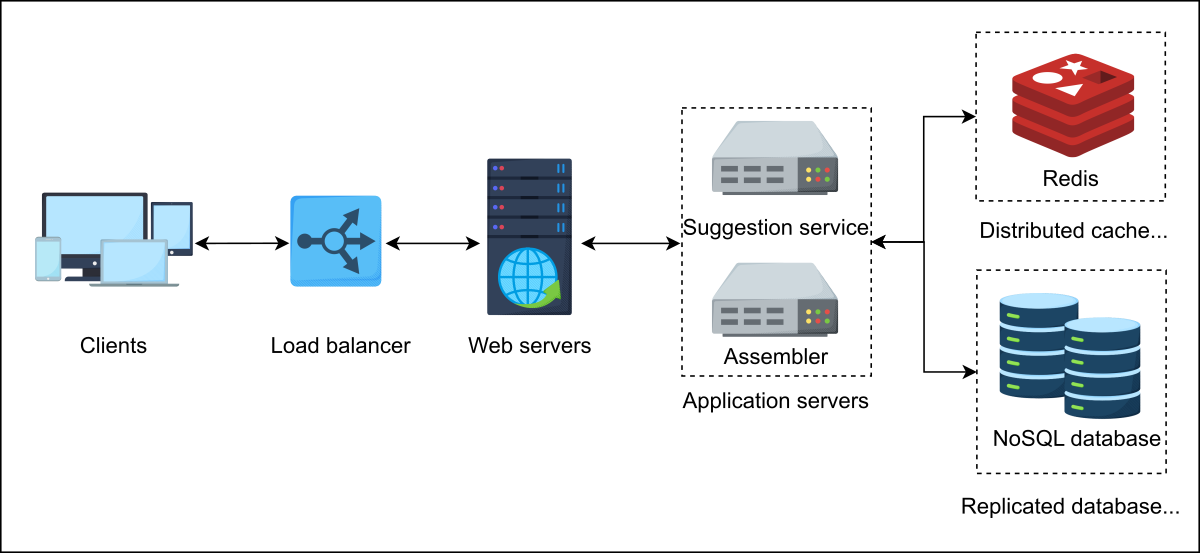
\includegraphics[width=0.5\textwidth]{Images/chapter_37/section_6376843531255808/4704341871427584.png}
 \caption{The high-level design of the typeahead suggestion system}
\end{figure}

Furthermore, we also need load balancers to distribute the incoming requests evenly. We also add web servers as entry points for clients so that they can forward requests to the appropriate microservices. These web servers encapsulate the internal system architecture and provide other services, such as authentication, monitoring, request shaping, management, and more.

\subsection{API design}\label{JthX2IMg3WoOdooxmp1kc}
\\
Since the system provides suggestions to the user and adds trending queries to the databases, we need the following APIs.

\subsubsection{Get suggestion}\label{ofuIFOCYBrS_Rj7JV1r42}

\begin{lstlisting}[language=JavaScript]
getSuggestions(prefix)
\end{lstlisting}

This API call retrieves suggestions from the servers. This call is made via the suggestion service and returns the response to the client.
\\
The following table explains the parameter that's passed to the API call:

\begin{table}[htbp]
\centering
\small
\adjustbox{max width=\textwidth}{
\begin{tabular}{|p{0.207\textwidth}|p{0.743\textwidth}|}
\hline
\textbf{Parameter} & \textbf{Description} \\
\hline
\hline
\texttt{prefix} & This refers to whatever the user has typed in the search bar. \\
\hline
\end{tabular}
}
\end{table}

\subsubsection{Add trending queries to the database}\label{bPgxm8QXvc5naPa0XaLaW}

\begin{lstlisting}[language=JavaScript]
addToDatabase(query)
\end{lstlisting}

This API call adds a trending \texttt{query} to the database via an assembler if the query has already been searched and has crossed a certain threshold.

\begin{table}[htbp]
\centering
\small
\adjustbox{max width=\textwidth}{
\begin{tabular}{|p{0.207\textwidth}|p{0.743\textwidth}|}
\hline
\textbf{Parameter} & \textbf{Description} \\
\hline
\hline
\texttt{query} & This represents a frequently searched query that crosses the predefined limit. \\
\hline
\end{tabular}
}
\end{table}

\begin{quote}
\textbf{Quiz:}
\textbf{Question 1:} Instead of updating the whole page, we just need to update the suggested query in the search box in real time. What technique can we use for this purpose?
\textbf{Answer:} We should update the query asynchronously using AJAX. AJAX is a set of web development techniques. It allows web pages to exchange a small amount of data, as in the typeahead suggestion system, with the server without interfering with the display and behaviors of the existing web page.
\end{quote}

Suppose our typeahead system needs to support multiple languages simultaneously to cater to a global user base. What are the potential bottlenecks in the current high-level design, and how will we solve them?
\\
To get started, say ``hello'' to Ed in the widget below, and it will lead the way.

In the next lesson, we'll learn about an efficient data structure that's used to store the suggestions or prefixes.



% End of section content